\documentclass[11pt]{report}
% PACKAGES
  \usepackage[a4paper,left=28mm,right=28mm,top=30mm,bottom=30mm]{geometry}
  \usepackage{graphicx,epstopdf}      % Used to import external graphics (figures)
  \usepackage{hyperref}       % Used for referring to links inside and outside the document
  \usepackage[table]{xcolor}  % To include colors 
  \usepackage{amsmath}        % For most of the math symbols and environments (such as \begin{align})
  \usepackage{amssymb}        % For using symbols in the document
  \usepackage{float}          % Arranging of figures on the page
  \usepackage[bf]{caption}    % Arranging the captions in floating environments [bf] makes the Figures bold
  \usepackage{subcaption}     % To arrange captions of subfigures
  \usepackage{booktabs}       % For standard tabular tables, with rules
  \usepackage{tabularx}       % For clean tables such as in the Nomenclature
  \usepackage{fancyhdr}       % Fancy headers
  % \usepackage[colorinlistoftodos]{todonotes}      % To create todo notes
  \usepackage[nottoc,notlot,notlof]{tocbibind}    % Add bibliography to content
  \usepackage{bm}             % Make bold symbols
  \usepackage{lipsum}
  \usepackage{parskip}
  \usepackage[export]{adjustbox}
  \usepackage{changepage}
% LAY-OUT
  % \usepackage{pdfpages}

  % \usepackage{pdflscape}

   \renewcommand\thesection{\arabic{section}}

  % \usepackage[mathletters]{ucs}
  % \usepackage[utf8x]{inputenc}
  %Bibliography for references, with reference style options
  \usepackage[
  backend=biber,
  bibstyle=ieee,
  citestyle=numeric-comp,
  dashed=false,
  url = false,
  maxnames=8,
  maxcitenames=2,
  mincitenames=1,
  sorting=none,
  isbn = false,
  doi = false
  ]{biblatex}
  \addbibresource{references.bib}

  %Set the page style
  \pagestyle{fancy}
  \fancyhead[L]{\ifodd\value{page} \slshape\nouppercase{\rightmark} \else \fi}
  \fancyhead[R]{\ifodd\value{page} \else \slshape\nouppercase{\leftmark} \fi}
  \chead{ }
  \lfoot{}
  \rfoot{}
  \cfoot{\small\thepage}


  %Give colors to links/refs etc
  \hypersetup{colorlinks, linkcolor={blue!0!black}, 
                          citecolor={blue!70!black}, 
                           urlcolor={blue!80!}} 
                       
  %% Set up numbering and spacing
  \numberwithin{equation}{section}        %Number the equations per section
  \numberwithin{figure}{section}          %Number the figures per section
  \numberwithin{table}{section}           %Number the tables per section
  \captionsetup[table]{skip=1pt}          %Skip 1 pt after a table
  \captionsetup[figure]{skip=3.5pt}       %Skip 4 pt after a figure
  \setcounter{secnumdepth}{3}             %Count up to the subsubsection 
  \setcounter{topnumber}{1}               %Number of floats at top of a page (default is 2)

  %%%%% proof/theorem/definition boxes

  \usepackage{cleveref}
  \usepackage[most]{tcolorbox}
  \newtcbtheorem{Theorem}{Theorem}{
    enhanced,
    sharp corners,
    attach boxed title to top left={
      yshifttext=-1mm
    },
    colback=white,
    colframe=blue!75!black,
    fonttitle=\bfseries,
    boxed title style={
      sharp corners,
      size=small,
      colback=blue!75!black,
      colframe=blue!75!black,
    } 
  }{thm}

  \newtcbtheorem{Definition}{Definition}{
    enhanced,
    sharp corners,
    attach boxed title to top left={
      yshifttext=-1mm
    },
    colback=white,
    colframe=blue!25,
    fonttitle=\bfseries,
    coltitle=black,
    boxed title style={
      sharp corners,
      size=small,
      colback=blue!25,
      colframe=blue!25,
    } 
  }{def}

  \newtcbtheorem[no counter]{Proof}{Proof}{
    enhanced,
    sharp corners,
    attach boxed title to top left={
      yshifttext=-1mm
    },
    colback=white,
    colframe=blue!25,
    fonttitle=\bfseries,
    coltitle=black,
    boxed title style={
      sharp corners,
      size=small,
      colback=blue!25,
      colframe=blue!25,
    } 
  }{prf}
% DEFINITIONS
  %% Titlepage definitions
  \newcommand{\deltitle}{Impact-Aware Control for a Dual-Arm Setup}      %Your project title
  \newcommand{\StudentName}{Gijs van den Brandt}  %Student name
  \newcommand{\StudentID}{1257110}                    %Your student number
  % \newcommand{\DCcode}{2021.109}                      %Get your DC code from the D&C secretariat

  %% Operators
  \DeclareMathOperator\sign{sgn}                      %Sign function
  \DeclareMathOperator\diag{diag}                     %Diagonal operator
  \DeclareMathOperator\imag{Imag}                     %Imaginary part of complex variable
  \DeclareMathOperator\real{Real}                     %Real part of complex variable
  \DeclareMathOperator*{\argmin}{\arg\!\min}          %Argmin operator
  \newcommand{\norm}[1]{\left\lVert#1\right\rVert}    %Norm operator

  %% Variable definition
  \newcommand{\R}{\mathbb{R}}                         % Set of real numbers
  \newcommand{\C}{\mathbb{C}}                         % Set of complex numbers

\begin{document}
\section*{Nomenclature}

$\begin{array}{l}
\text{\textbf{Joint space}}\\
q \;\quad \text{Joint positions}\\
M \;\quad \text{Inertia matrix}\\
\\
\text{\textbf{Posture task space}}\\
\beta \quad \text{Desired acceleration of the first joint } q_1\\
k \;\quad \text{Posture stiffness}\\

\\
\text{\textbf{Impedance task space} (all variables are expressed in world frame)}\\
R \quad \text{Rotation matrix of the end effector}\\
\omega \quad \text{Angular velocity vector of the end effector}\\
\alpha \quad \text{Angular acceleration vector of the end effector}\\
p \;\quad \text{Position vector of the end effector}\\
v \;\quad \text{Linear velocity vector of the end effector}\\
a \;\quad \text{Linear acceleration vector of the end effector}\\
f \;\quad \text{Virtual wrench vector acting on the end effector}\\
K \quad \text{Impedance stiffness matrix} \\
\Lambda \;\quad \text{Impedance inertia matrix} \\
\\

\text{\textbf{Reference Spreading}}\\
\varphi  \quad \text{Time of impact}\\
\gamma  \quad \text{Impact time-based interpolation variable}\\
T  \quad \text{Duration of interim impact mode}\\
m \quad \text{Intermediate impact mode(0: no RS, 1: Jari, 2: Sven, 3: mixing)}\\\\
\text{\textbf{Sub- and superscripts}}\\
(\cdot)^{a} \quad \text{Ante-impact signal}\\
(\cdot)^{p} \quad \text{Post-impact signal}\\
(\cdot)_{dem} \quad \text{Signals from VR device during recording}\\
(\cdot)_{rec} \;\quad \text{Signals measured from robot or calculated during recording}\\
(\cdot)_{ref} \;\quad \text{Signals determined using RS scheme}\\
(\cdot)_{rep} \;\quad \text{Signals measured from robot or calculated during replay}\\
\end{array}$
\newpage
\section*{Recording}

$\begin{array}{l}
\ddot{q}_{rec} = \min_{\ddot{q}}\left \|  \begin{bmatrix}
\alpha(\ddot{q})\\ 
a(\ddot{q})
\end{bmatrix} - \Lambda^{-1}f_{rec} \right \| + \left \| \ddot{q}_1-\beta_{rec} \right \|\\\\
f_{rec} =2(\Lambda K_{rec})^{\frac{1}{2}} \begin{bmatrix}
\omega_{dem} - \omega_{rec}
\\ 
v_{dem}-v_{rec}
\end{bmatrix} + K_{rec} \begin{bmatrix}
R_{rec}(\log({R_{rec}}^TR_{dem}))^{\vee }\\ 
p_{dem}-p_{rec}
\end{bmatrix}\\\\
\beta_{rec} = 2\sqrt{k_{rec}}\left [ -\dot{q}_{1,rec}  \right ] + k_{rec}\left [ -q_{1,rec}  \right ]

\end{array}$\\
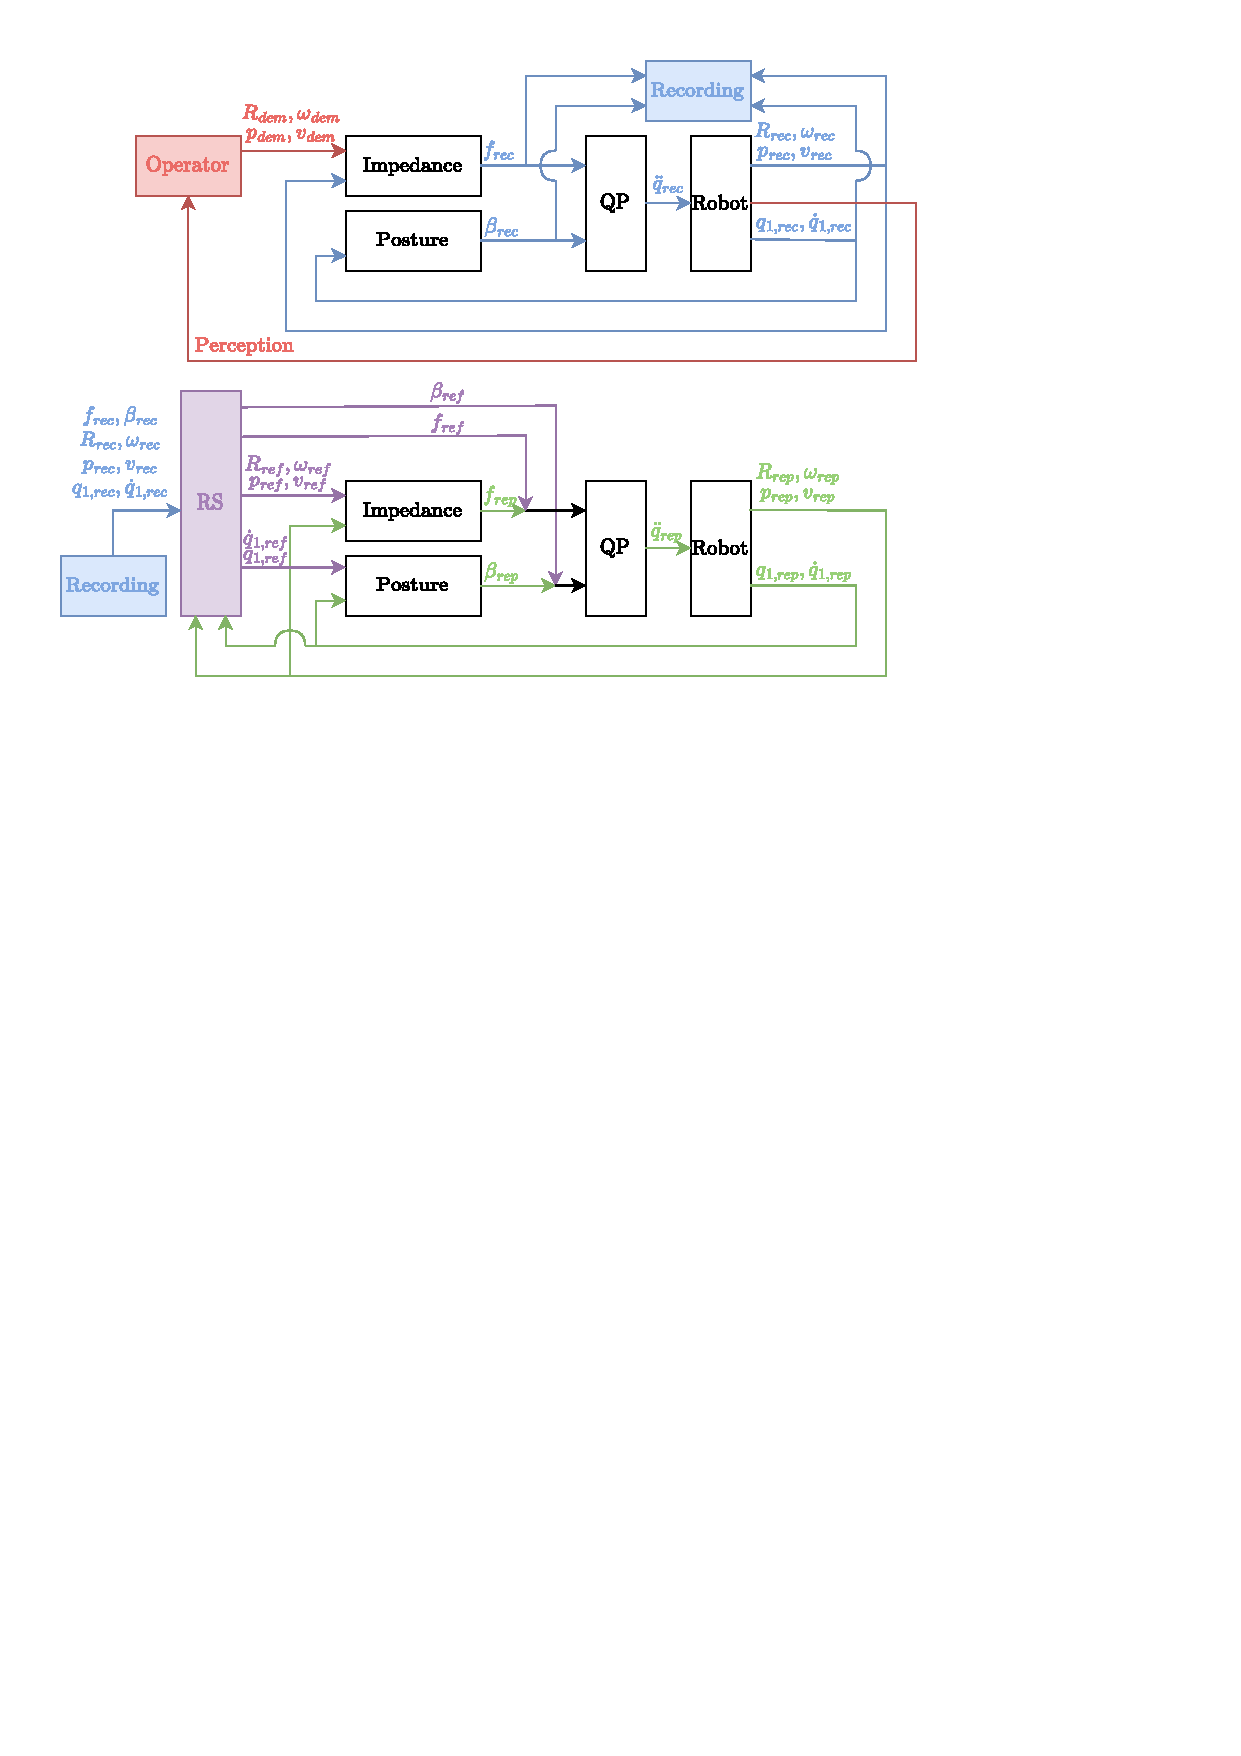
\includegraphics[trim={1cm 23.3cm 5cm 1cm}, clip]{Graphics/qp.pdf}\\
\section*{Reference Extending}
$\begin{array}{l}
REhold(x,t,\varphi) 
% = \begin{bmatrix} x^a(t) & x^p(t) \end{bmatrix} 
= \begin{cases} 
\begin{bmatrix} x(t) & x(\varphi) \end{bmatrix},& \text{if } t\leq \varphi\\
\begin{bmatrix} x(\varphi) & x(t) \end{bmatrix},& \text{if } t> \varphi\\
\end{cases}\\\\\\

REintegrate(x,y,t,\varphi) 
% = \begin{bmatrix} y^a(t) & y^p(t) \end{bmatrix} 
= \begin{cases} 
\begin{bmatrix} x(t) & x(\varphi) \end{bmatrix}+\begin{bmatrix}0 & y(\varphi)(t-\varphi) \end{bmatrix},& \text{if } t\leq \varphi\\
\begin{bmatrix} x(\varphi) & x(t) \end{bmatrix}+\begin{bmatrix}y(\varphi)(t-\varphi) & 0  \end{bmatrix},& \text{if } t> \varphi\\
\end{cases}\\\\

\begin{bmatrix} R_{rec}^a(t) & R_{rec}^p(t) \end{bmatrix} 
= \begin{cases} 
\begin{bmatrix} R_{rec}(t) & R_{rec}(\varphi_{rec})e^{\omega_{rec}(\varphi_{rec})(t-\varphi_{rec})} \end{bmatrix},& \text{if } t\leq  \varphi_{rec}\\
\begin{bmatrix} R_{rec}(\varphi_{rec})e^{\omega_{rec}(\varphi_{rec})(t-\varphi_{rec})} & R_{rec}(t) \end{bmatrix},& \text{if } t> \varphi_{rec}\\
\end{cases}\\

\begin{bmatrix} p_{rec}^a(t) & p_{rec}^p(t) \end{bmatrix} = REintegrate(p_{rec},\dot{q}_{1,rec},t,\varphi_{rec})\\
\begin{bmatrix} q_{1,rec}^a(t) & q_{1,rec}^p(t) \end{bmatrix} = REintegrate(q_{1,rec},\dot{q}_{1,rec},t,\varphi_{rec})\\


\begin{bmatrix} f_{rec}^a(t) & f_{rec}^p(t) \end{bmatrix} = REhold(f_{rec},t,\varphi_{rec})\\
\begin{bmatrix} \beta_{rec}^a(t) & \beta_{rec}^p(t) \end{bmatrix} = REhold(\beta_{rec},t,\varphi_{rec})\\
\begin{bmatrix} v_{rec}^a(t) & v_{rec}^p(t) \end{bmatrix} = REhold(v_{rec},t,\varphi_{rec})\\
\begin{bmatrix} \omega_{rec}^a(t) & \omega_{rec}^p(t) \end{bmatrix} = REhold(\omega_{rec},t,\varphi_{rec})\\
\begin{bmatrix} \dot{q}_{1,rec}^a(t) & \dot{q}_{1,rec}^p(t) \end{bmatrix} = REhold(\dot{q}_{1,rec},t,\varphi_{rec})
\end{array}$

\section*{Reference Switching}

$\begin{array}{l}
\gamma_{rep} = \frac{t-\varphi_{rep}}{T}\\

RS(x^a(t),x^p(t),t,\gamma) = \begin{cases} 
x^a,& \text{if } \gamma \leq 0\\
x^p,& \text{if } \gamma \geq 1\\

x^p,& \text{if } (0< \gamma < 1)\wedge(m=0)\\ 
x^a,& \text{if } (0< \gamma < 1)\wedge(m=1)\\ 
x^a,& \text{if } (0< \gamma < 1)\wedge(m=2)\\ 
(1-\gamma)x^a+ \gamma x^p,& \text{if } (0< \gamma < 1)\wedge(m=3)\\ \end{cases}\\\\



RSvel(x,x^a(t),x^p(t),t,\gamma) = \begin{cases} 
x^a,& \text{if } \gamma \leq 0\\
x^p,& \text{if } \gamma \geq 1\\

x^p,& \text{if } (0< \gamma < 1)\wedge(m=0)\\ 
x,& \text{if } (0< \gamma < 1)\wedge(m=1)\\ 
0,& \text{if } (0< \gamma < 1)\wedge(m=2)\\ 
\gamma x^p,& \text{if } (0< \gamma < 1)\wedge(m=3)\\ 
\end{cases}\\\\

RScont(x^a(t),x^p(t),t,\gamma) = RSvel(0,x^a(t),x^p(t),t,\gamma) + \begin{cases} 
x^a,& \text{if } (0< \gamma < 1)\wedge(m=1)\\ 
x^a,& \text{if } (0< \gamma < 1)\wedge(m=2)\\ 
(1-\gamma)x^a,& \text{if } (0< \gamma < 1)\wedge(m=3)\\
0 ,& \text{otherwise}\\ \end{cases}\\\\

f_{ref} = RS(f_{rec}^a, f_{rec}^p,t,\gamma_{rep})\\
\beta_{ref} = RS(\beta_{rec}^a, \beta_{rec}^p,t,\gamma_{rep})\\
p_{ref} = RS(p_{rec}^a, p_{rec}^p,t,\gamma_{rep})\\
q_{1,ref} = RS(q_{1,rec}^a, q_{1,rec}^p,t,\gamma_{rep})\\


\dot{q}_{1,ref} = RSvel(\dot{q}_{1,rep},\dot{q}_{1,rec}^a, \dot{q}_{1,rec}^p,t,\gamma_{rep})\\

v_{ref} = RSvel(v_{rep},v_{rec}^a, v_{rec}^p,t,\gamma_{rep})\\
\alpha_{ref} = RSvel(\alpha_{rep},\alpha_{rec}^a, \alpha_{rec}^p,t,\gamma_{rep})\\
R_{ref} = 
\begin{cases} 
R^a_{rec},& \text{if } \gamma \leq 0\\
R_{rec}^p,& \text{if } \gamma \geq 1\\

R_{rec}^p,& \text{if } (0< \gamma < 1)\wedge(m=0)\\ 
R_{rep},& \text{if } (0< \gamma < 1)\wedge(m=1)\\ 
I,& \text{if } (0< \gamma < 1)\wedge(m=2)\\ 
R_{rep}(R_{rep}^TR_{rec})^\gamma,& \text{if } (0< \gamma < 1)\wedge(m=3)\text{Klopt deze interpolatie???}\\ 
\end{cases}\\\\
% definition
% - ff: f, beta
% - velocities: dq_1, v, alpha, 
% - positions: p, q_1
% - rotations: R

% RE:
% - ff, velocities: hold
% - position: integrate
% - rotations: :)

% Rs:
% - ff, positions: default
% - velocities: hold
% - rotations: :)

\end{array}$

\newpage
\section*{Replaying}
$\begin{array}{l}
\ddot{q}_{rep} = \min_{\ddot{q}}\left \|  \begin{bmatrix}
\alpha(\ddot{q})\\ 
a(\ddot{q})
\end{bmatrix} - \Lambda^{-1}(f_{rep}+f_{rec}) \right \| + \left \|\ddot{q}_1-(\beta_{rep}+\beta_{rec}) \right \|\\\\
f_{rep} =2(\Lambda K_{rep})^{\frac{1}{2}} \begin{bmatrix}
\omega_{rec} - \omega_{rep}
\\ 
v_{rec}-v_{rep}
\end{bmatrix} + K_{rep} \begin{bmatrix}
R_{rep}(\log({R_{rep}}^TR_{rec}))^{\vee }\\ 
p_{rec}-p_{rep}
\end{bmatrix}\\\\
\beta_{rep} = 2\sqrt{k_{rep}}\left [ \dot{q}_{1,rec}-\dot{q}_{1,rep}  \right ] + k_{rep}\left [ q_{1,rec}-q_{1,rep}  \right ]
\end{array}$

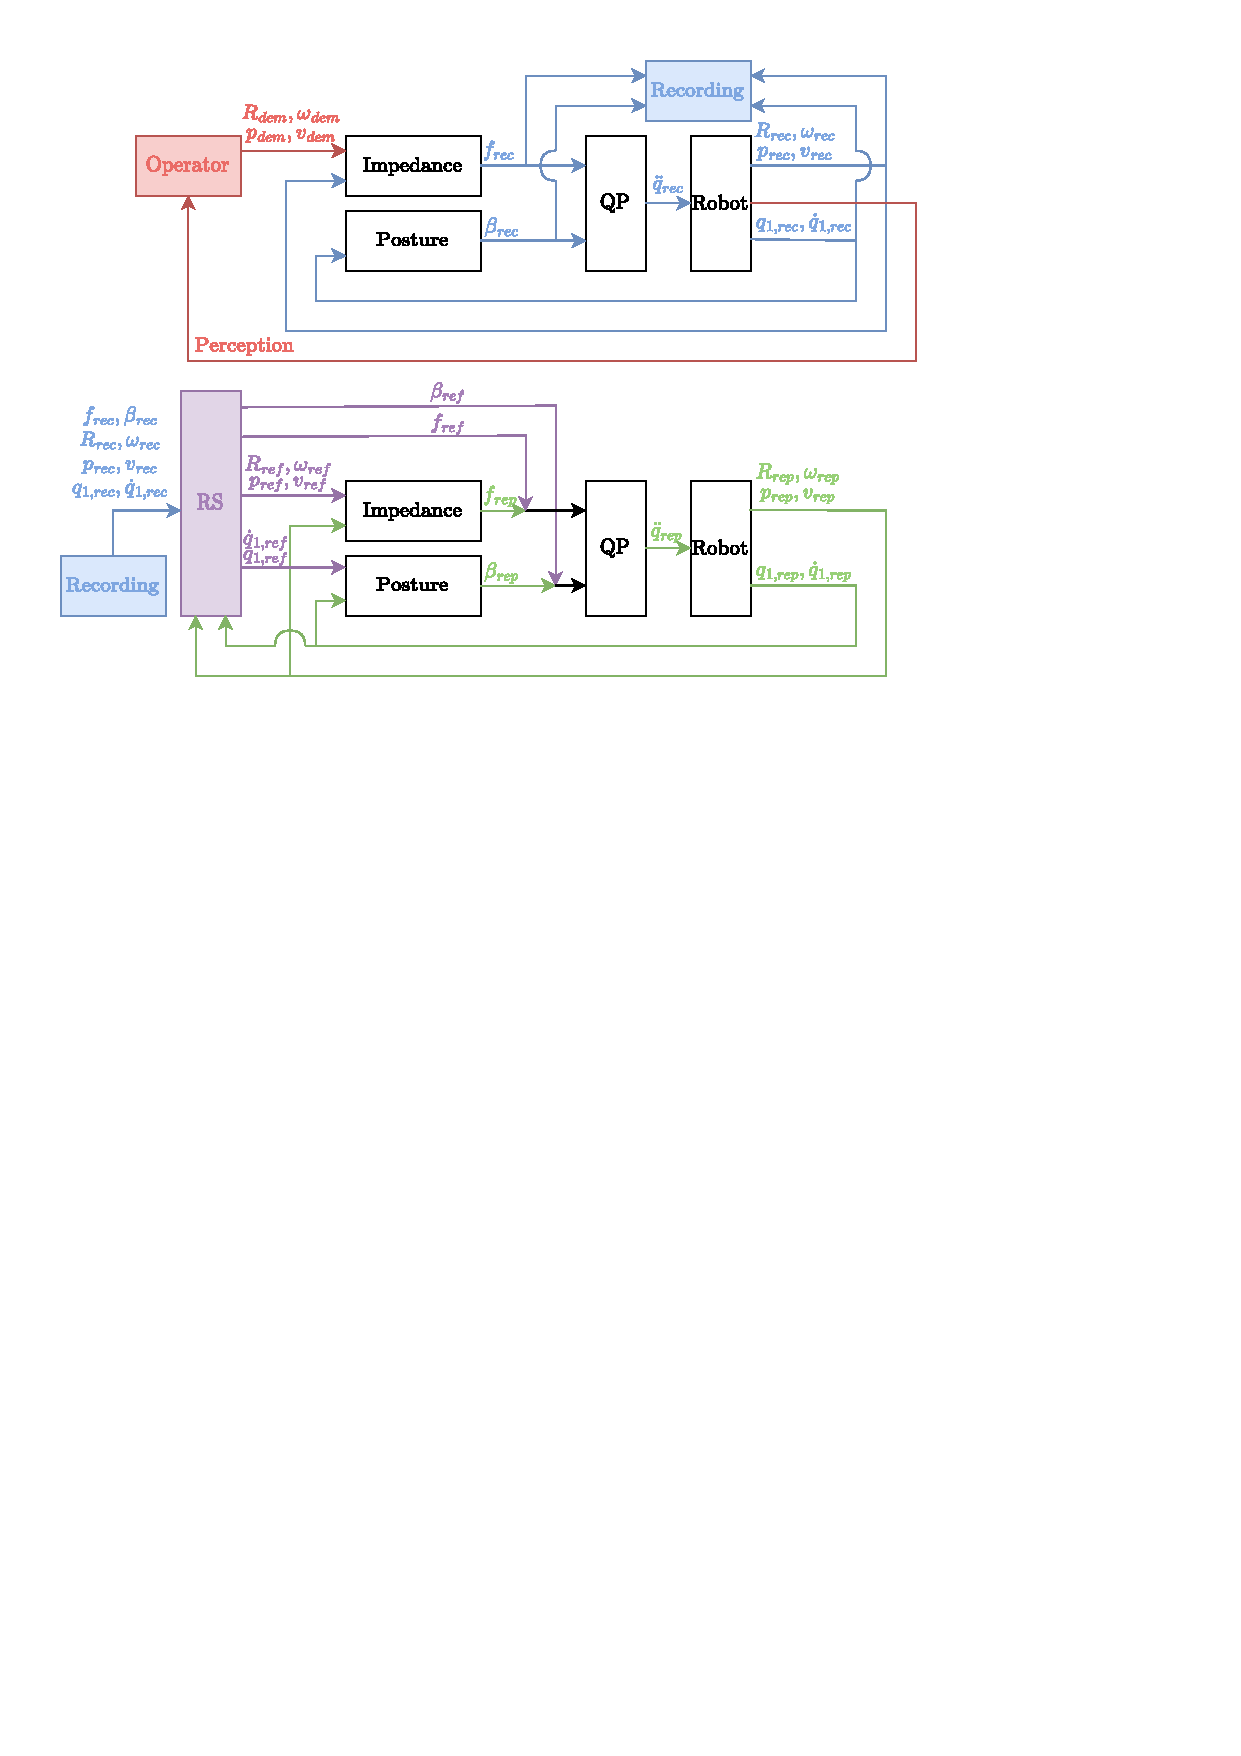
\includegraphics[trim={1cm 17.8cm 5cm 6.5cm}, clip]{Graphics/qp.pdf}

\section*{Miscelaneous}
$\begin{array}{l}
\begin{bmatrix}
\omega\\ 
v
\end{bmatrix} = J\dot{q}\\\\
\begin{bmatrix}
\alpha(\ddot{q})\\ 
a(\ddot{q})
\end{bmatrix} = J\ddot{q} + \dot{J}\dot{q}\\\\
\Lambda^{-1} = J^TM^{-1}J
\end{array}$

\end{document}